%%
%% This is file `sample-sigconf.tex',
%% generated with the docstrip utility.
%%
%% The original source files were:
%%
%% samples.dtx  (with options: `sigconf')
%% 
%% IMPORTANT NOTICE:
%% 
%% For the copyright see the source file.
%% 
%% Any modified versions of this file must be renamed
%% with new filenames distinct from sample-sigconf.tex.
%% 
%% For distribution of the original source see the terms
%% for copying and modification in the file samples.dtx.
%% 
%% This generated file may be distributed as long as the
%% original source files, as listed above, are part of the
%% same distribution. (The sources need not necessarily be
%% in the same archive or directory.)
%%
%% The first command in your LaTeX source must be the \documentclass command.
\documentclass[sigconf]{acmart}

%%%% As of March 2017, [siggraph] is no longer used. Please use sigconf (above) for SIGGRAPH conferences.

%%%% As of May 2020, [sigchi] and [sigchi-a] are no longer used. Please use sigconf (above) for SIGCHI conferences.

%%%% Proceedings format for SIGPLAN conferences 
% \documentclass[sigplan, anonymous, review]{acmart}

%%%% Proceedings format for conferences using one-column small layout
% \documentclass[acmsmall,review]{acmart}

%%
%% \BibTeX command to typeset BibTeX logo in the docs
\AtBeginDocument{%
  \providecommand\BibTeX{{%
    \normalfont B\kern-0.5em{\scshape i\kern-0.25em b}\kern-0.8em\TeX}}}

%% Rights management information.  This information is sent to you
%% when you complete the rights form.  These commands have SAMPLE
%% values in them; it is your responsibility as an author to replace
%% the commands and values with those provided to you when you
%% complete the rights form.
\setcopyright{acmcopyright}
\copyrightyear{2018}
\acmYear{2018}
\acmDOI{10.1145/1122445.1122456}

%% These commands are for a PROCEEDINGS abstract or paper.
\acmConference[Woodstock '18]{Woodstock '18: ACM Symposium on Neural
  Gaze Detection}{June 03--05, 2018}{Woodstock, NY}
\acmBooktitle{Woodstock '18: ACM Symposium on Neural Gaze Detection,
  June 03--05, 2018, Woodstock, NY}
\acmPrice{15.00}
\acmISBN{978-1-4503-XXXX-X/18/06}


%%
%% Submission ID.
%% Use this when submitting an article to a sponsored event. You'll
%% receive a unique submission ID from the organizers
%% of the event, and this ID should be used as the parameter to this command.
%%\acmSubmissionID{123-A56-BU3}

%%
%% The majority of ACM publications use numbered citations and
%% references.  The command \citestyle{authoryear} switches to the
%% "author year" style.
%%
%% If you are preparing content for an event
%% sponsored by ACM SIGGRAPH, you must use the "author year" style of
%% citations and references.
%% Uncommenting
%% the next command will enable that style.
%%\citestyle{acmauthoryear}

%%
%% end of the preamble, start of the body of the document source.
\begin{document}

%%
%% The "title" command has an optional parameter,
%% allowing the author to define a "short title" to be used in page headers.
\title{INForex: An Interactive News Digestion for Forex Investors}

%%
%% The "author" command and its associated commands are used to define
%% the authors and their affiliations.
%% Of note is the shared affiliation of the first two authors, and the
%% "authornote" and "authornotemark" commands
%% used to denote shared contribution to the research.

\author{Chih-Hen Lee}
\authornote{Both authors contributed equally to this work.}
\email{ch.lee@citi.sinica.edu.tw}
\affiliation{%
  \institution{Research Center for Information Technology Innovation, Academia Sinica}
  \city{Taipei}
  \country{Taiwan}}

\author{Yi-Shyuan Chiang}
\authornotemark[1]
\email{yschiang@gapp.nthu.edu.tw}
\affiliation{%
  \institution{Research Center for Information Technology Innovation, Academia Sinica}
  \city{Taipei}
  \country{Taiwan}}

\author{Chuan-Ju Wang}
\email{cjwang@citi.sinica.edu.tw}
\affiliation{%
  \institution{Research Center for Information Technology Innovation, Academia Sinica}
  \city{Taipei}
  \country{Taiwan}}


%%
%% By default, the full list of authors will be used in the page
%% headers. Often, this list is too long, and will overlap
%% other information printed in the page headers. This command allows
%% the author to define a more concise list
%% of authors' names for this purpose.
\renewcommand{\shortauthors}{Lee, Chiang and Wang}

%%
%% The abstract is a short summary of the work to be presented in the
%% article.
\begin{abstract}
Foreign exchange (Forex) markets reflect real-world events, locally or globally.
Thus,  financial news is oftentimes leveraged for predicting the trends of Forex.
In this demonstration, we propose INForex, an interactive web-based system that displays a Forex plot alongside with related financial news.
To our best knowledge, this is the first system that successfully aligns the presentation of two types of time-series data: the Forex data and the textual news data in a unified and time-aware manner. 
Specifically, we first present two event detection methods based on the standard deviation (SD) and directional change (DC) of the Forex data and use them to locate specific periods when the prices or trends in Forex markets dramatically change.
Moreover, INForex comes with a keyword filtering function that allows users to filter news with self-defined keywords.
The system can be of great help in revealing valuable insights and relations between two types of time-series data and thus be valuable for decision making for not only professional financial analysts or traders but also common investors.
The system is now online available at ~\url{http://chlee.pythonanywhere.com/forex/}.
\end{abstract}

%%
%% The code below is generated by the tool at http://dl.acm.org/ccs.cfm.
%% Please copy and paste the code instead of the example below.
%%
\begin{CCSXML}
<ccs2012>
   <concept>
       <concept_id>10002951.10003260.10003282</concept_id>
       <concept_desc>Information systems~Web applications</concept_desc>
       <concept_significance>500</concept_significance>
       </concept>
 </ccs2012>
\end{CCSXML}

\ccsdesc[500]{Information systems~Web applications}


%%
%% Keywords. The author(s) should pick words that accurately describe
%% the work being presented. Separate the keywords with commas.
\keywords{Forex, financial news, standard deviation, directional change}

%% A "teaser" image appears between the author and affiliation
%% information and the body of the document, and typically spans the
%% page.
\begin{teaserfigure}
  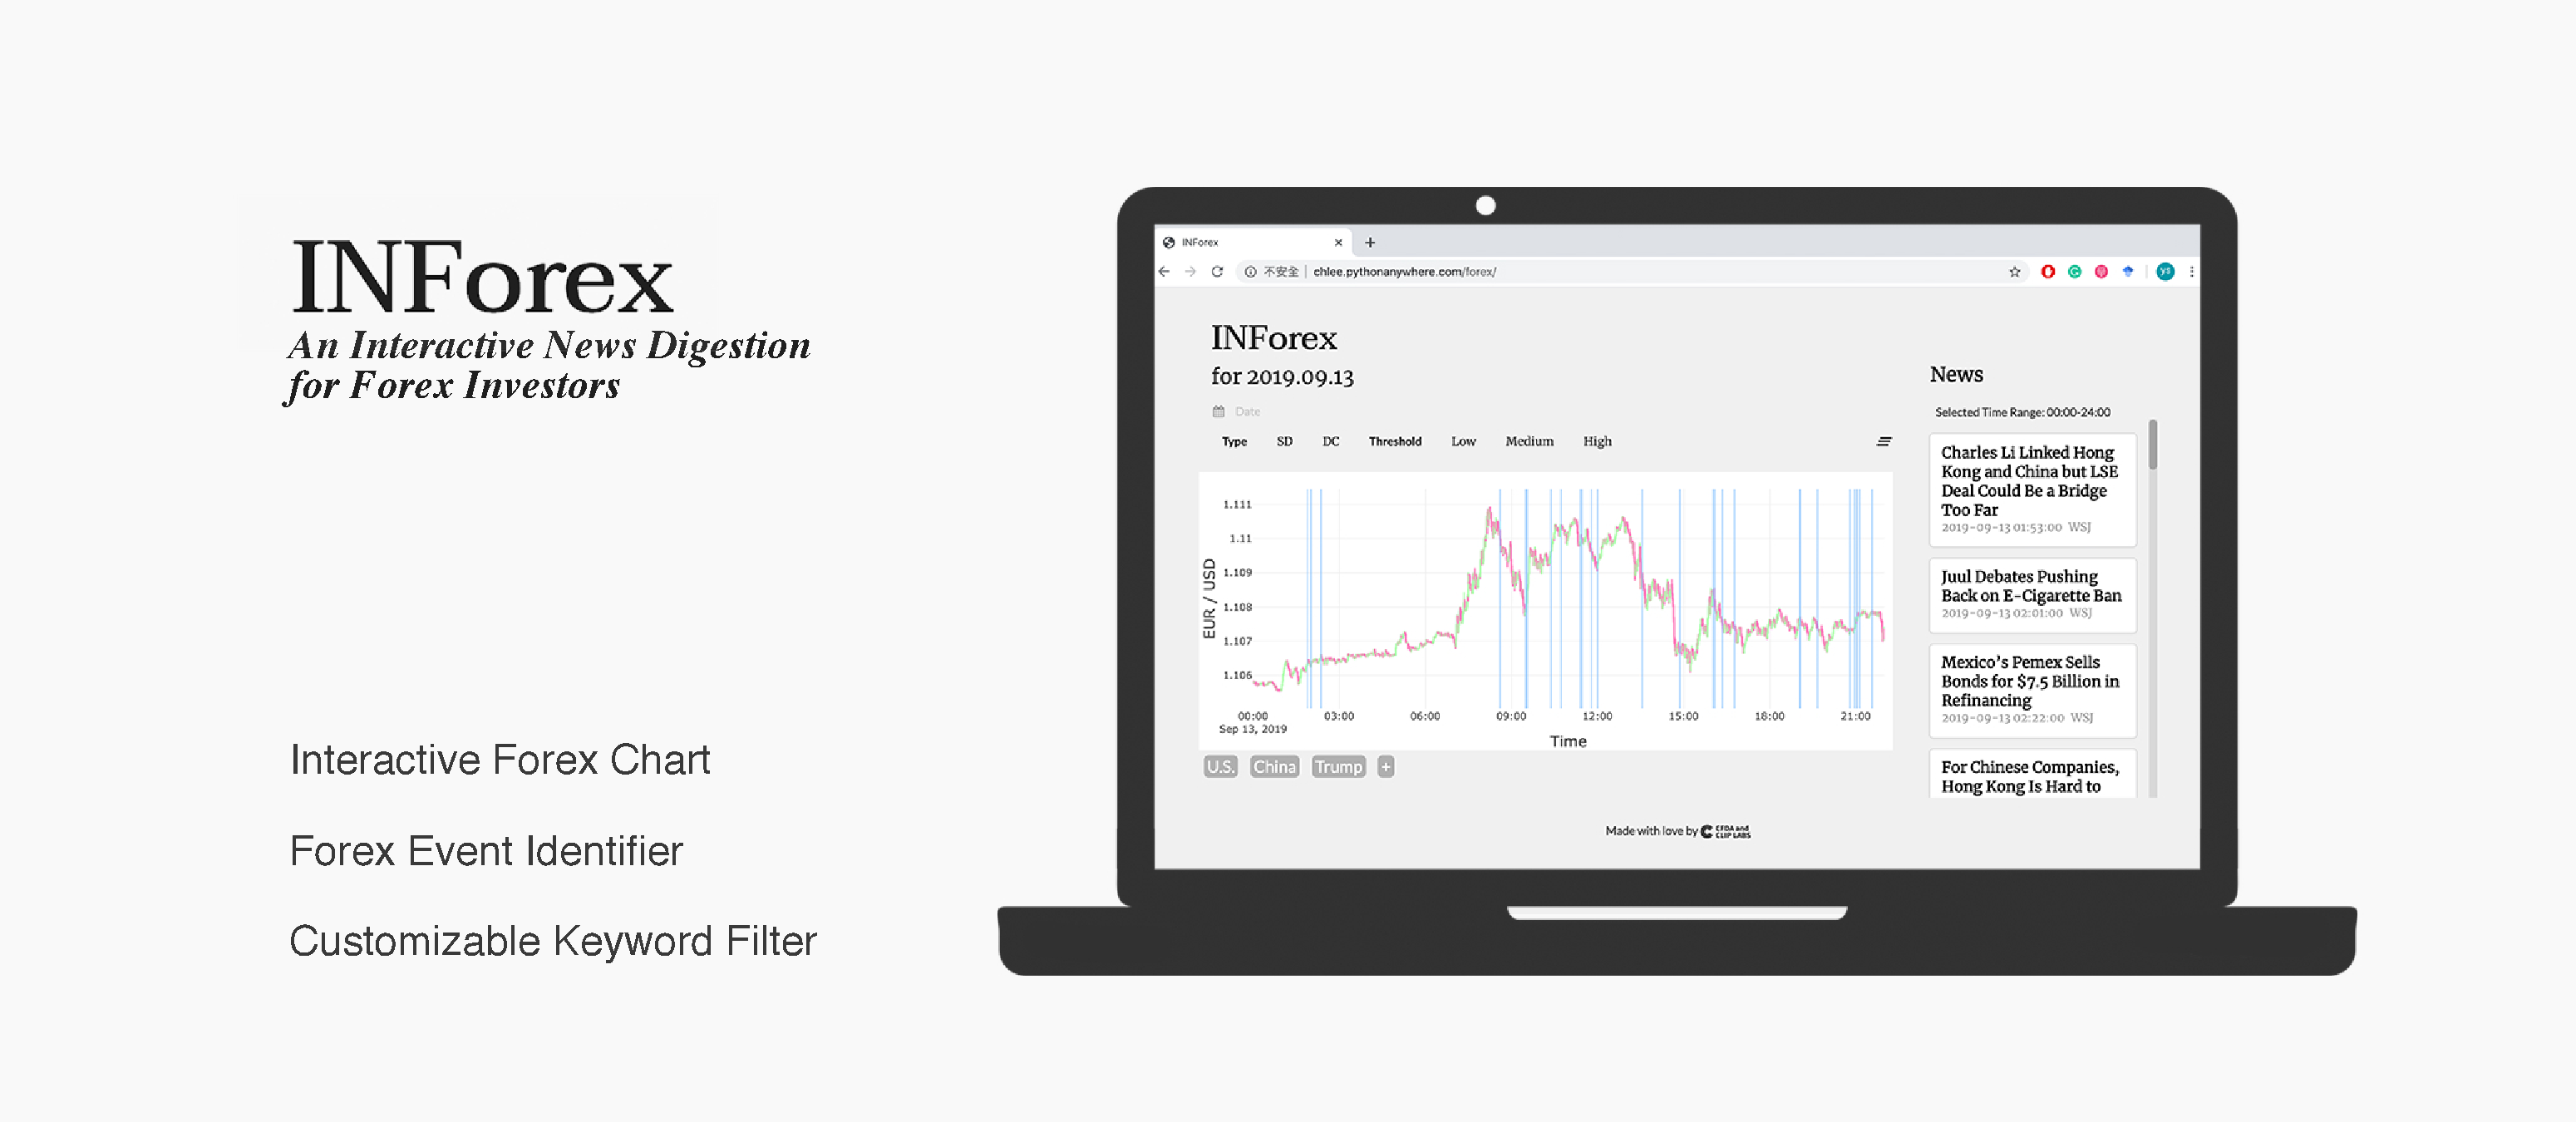
\includegraphics[width=\textwidth]{teaser.pdf}
  \caption{INForex available at~\url{http://chlee.pythonanywhere.com/forex/}.}
  \Description{}
  \label{fig:teaser}
\end{teaserfigure}


%%
%% This command processes the author and affiliation and title
%% information and builds the first part of the formatted document.
\maketitle

\section{Introduction}
Foreign exchange (Forex) market has been one of the most popular financial markets for decades, with an estimated \$1\ trillion traded every day~\cite{YAO200079}.
Spot trading, currency options, currency futures, and currency exchange-traded funds (ETFs) are four major ways to trade Forex~\cite{TradeForex}.
The strategies might vary but they are driven by an intuitive rule of thumb, which is to buy low and sell high~\cite{KOOLEN2014144,Zervos11}.
Therefore, whether investors can accurately forecast the prices or trends is extremely crucial. 

Forex markets are influenced by numerous factors, such as producer price index (PPI), interest rates, and politics.
In order to consider as many factors as possible to have more comprehensive views for Forex investment, most investors rely on news for them to stay informed.
Besides the fact that news usually reflect the real-world events, the similar nature of news and Forex also makes these two co-dependent.
For example, if the Federal Reserve System (Fed) cuts the interest rate, it is more likely that the value of USD would drop; also, such a devaluation would later make another piece of news~\cite{"CNBC"}. 

Considering the critical roles of news for Forex investment, in this demonstration, we propose INForex, an interactive web-based system that displays a Forex plot alongside with related financial news.
The proposed system aims to highlight the connection between two types of time-series data: the Forex and the news data by aligning the timing of them.
INForex is designed to display the news' release time as vertical lines on the Forex plot to emphasize the order of breaking news and exchange rates. In addition, when users hover on a vertical line, the background colour of the corresponding news would change. 
Moreover, we propose to use two event detection methods based on the standard deviation (SD) and directional change (DC)~\cite{7850020} of the Forex data to locate specific periods when the prices or trends in Forex markets dramatically change.
Via this design, user can pay more attention to the changes of trend or where the prices have larger volatility.
Finally, INForex comes with a keyword filtering function that allows users to filter news with self-defined keywords.
To our best knowledge, this is the first system that effectively visualizes two types of time-series data: the Forex data and the textual news data in a unified and time-aware manner. 
The proposed INForex can be of great help in revealing valuable insights and relations between two types of time-series data and thus be valuable for decision making for not only professional financial analysts or traders but also common investors.

The remainder of this paper is organized as follows.
In Section~\ref{sec:related}, we review previous studies related to Forex and news and major websites for Forex traders.
Section~\ref{sec:system} describes the proposed system with details related to data collection, event detection algorithms, interfaces and key features.
After that, we provide a case study in section~\ref{sec:case} and Section~\ref{sec:conclude} provides the conclusion and future work.

\section{Related Work and Systems}\label{sec:related}
The dynamics between news and Forex markets have been explored from several different aspects.
Evans and Lyons (2005) prove that news can have significant effects on currency for days~\cite{EVANS2005197}, and macro news can affect currency prices directly and indirectly via order flow~\cite{EVANS200826}.
There is also more evidence showcasing news and Forex trend are correlated.
For instance, Bauwens et al.  (2005) show that volatility increases right before the announcement of scheduled news and unscheduled-but-periodic news~\cite{BAUWENS20051108}, while Chatrath et al. (2014) suggest that prices respond quickly within 5-min after the news release~\cite{CHATRATH201442}.
With how Forex markets and news interact in mind, it is reasonable for traders to begin their days by reading news commentary to determine the market sentiment and the direction for trading~\cite{samuels2015trader}.

Apart from the literature discussing the relation between Forex and news, there are many trading websites which provide useful information for Forex investors, each of which has its own features and limitations~\cite{ForexWebsites}.
For instance, BabyPips\footnote{\url{https://www.babypips.com}} is a friendly website for junior traders, providing not only Forex plots but also courses, tutorials and forums for beginners. Bloomberg\footnote{\url{https://www.bloomberg.com}} is a well-known news agency; thus, in addition to currency data and plots, it also provides various categories of news for users to focus on their interest.
TradingView\footnote{\url{https://www.tradingview.com}} provides numerous functions in a page, such as watchlist, alerts, headlines and real-time chats, where users can customize the settings. 
However, most of these websites do not put the news and Forex plot at the same page or do not explicitly align the news releasing time with the Forex prices.
Most of them neglect the time-dependent relation between news and Forex data and thus do not effectively visualizes two types of time-series data in a unified and time-aware manner. 


\section{System Description}\label{sec:system}

\subsection{Data Collection}
The Forex data was collected from philipperemy/FX-1-Minute-Data.\footnote{\url{https://github.com/philipperemy/FX-1-Minute-Data}}
For demonstration purpose, we chose the EUR/USD index and used the DateTime Stamp, OPEN Bid Quote, HIGH Bid Quote, LOW Bid Quote and CLOSE Bid Quote columns to plot the Forex candlestick chart; moreover, the time span for the Forex data is from August 4, 2019 to September 13, 2019, and the granularity of data is minute. 
As for the news, we crawled the data from The Wall Street Journal,\footnote{\url{https://www.wsj.com}} each of which contains the title, the source, the release time, and the corresponding url.
In this demonstration, there are 1,116 news in total.

\subsection{Event Detection Algorithms}\label{sec:algo}
The proposed system comes with two event detection algorithms: one is based on the standard deviation of Forex price differences (referred as SD events hereafter) and one is based on the directional change of Forex prices (referred as DC events hereafter)~\cite{7850020}. 
Specifically, SD events indicate the time points where the Forex prices dramatically change, whereas DC events show the time points where the trends of Forex prices change.

We here briefly describe the two algorithms.
Let $P= [p_1, p_2, ..., p_n]$ denote a series of Forex prices, where $p_t$ stands for the CLOSE Bid Quote at minute $t$ and $n$ equals to the total numbers of daily Forex data; also, the series of difference rates between two Forex prices is defined as $\mathcal{D}= [d_1, d_2, ..., d_m]$, where $d_t = {(p_{t+w}-p_t)}/{p_t}$ and $w\in\mathbb Z^+$ denotes the range in minutes.
Note that we set $w=30$ in our prototype system.
We first calculate the standard deviation of differences in list $\mathcal{D}$ and denoted it as $\sigma_\mathcal{D}$; we then use the $z$-score of each difference to determine the event events (i.e., $z_{d_i}=(|d_i-m_{\mathcal{D}}|)/\sigma_{\mathcal{D}}>\tau$) , where $m_{\mathcal{D}}$ denotes the mean of the list $\mathcal{D}$.)
In this demonstration, we consider $\tau=1,2,3$ as our thresholds that correspond to the label \emph{Low}, \emph{Medium}, and \emph{High} in the system. 
Note that a higher threshold locates less events.

As for the DC events, the market is summarized into a set of uptrend and downtrend events~\cite{7850020}.
A DC event, including a start point and an end point, can be seen as a period that the trend starts to change.
At first, we let the first element in the price list $p_1$ as a starting point of the algorithm; then, the algorithm starts looking through the price list $P$ in a sequential manner until it locates a price $p_c$ that $|{(p_c-p_1)}/{p_1}|>\theta$.
In this demonstration, we consider $\theta=\sigma_{\mathcal{D}},2\sigma_{\mathcal{D}},3\sigma_{\mathcal{D}}$ as our thresholds that as well as correspond to the label \emph{Low}, \emph{Medium}, and \emph{High} in the system.
If $p_c > p_1$, the span from $p_1$ to $p_c$ denotes an upward DC event; otherwise, it is a downward DC event.
After finding the first DC event, we start to locate other DC events in the rest of the price sequence.
Let us consider a market starts with a downtrend, meaning that the Forex market is now in a downtrend and waiting for a next uptrend, for which we keep updating the lowest price $p_\ell$ in this downtrend until we find a price $p_k$ that ${(p_k-p_\ell)}/{p_\ell}>\theta$. Then, we mark that the span from $p_\ell$ to $p_k$ is an upward DC event, and the trend becomes upward.
Similarly, if a market is in an uptrend, we keep updating the highest price $p_h$ in this uptrend until we find a price $p_k$ that ${(p_h-p_k)}/{p_h}>\theta$, then the ``$p_h$-to-$p_c$'' spans a downward DC event, and the trend becomes downward.
After finishing looking through all daily Forex data, we obtain a series of DC events.




\subsection{Interfaces and features}
The interface of INForex can be divided into two main parts: 1) a Forex chart (in the left panel of the system) and 2) the news section (in the right panel of the system).
Users are allowed to customize the selection criteria either by directly manipulating the Forex chart or applying the keyword filters.

\begin{figure}[h]
  \centering
  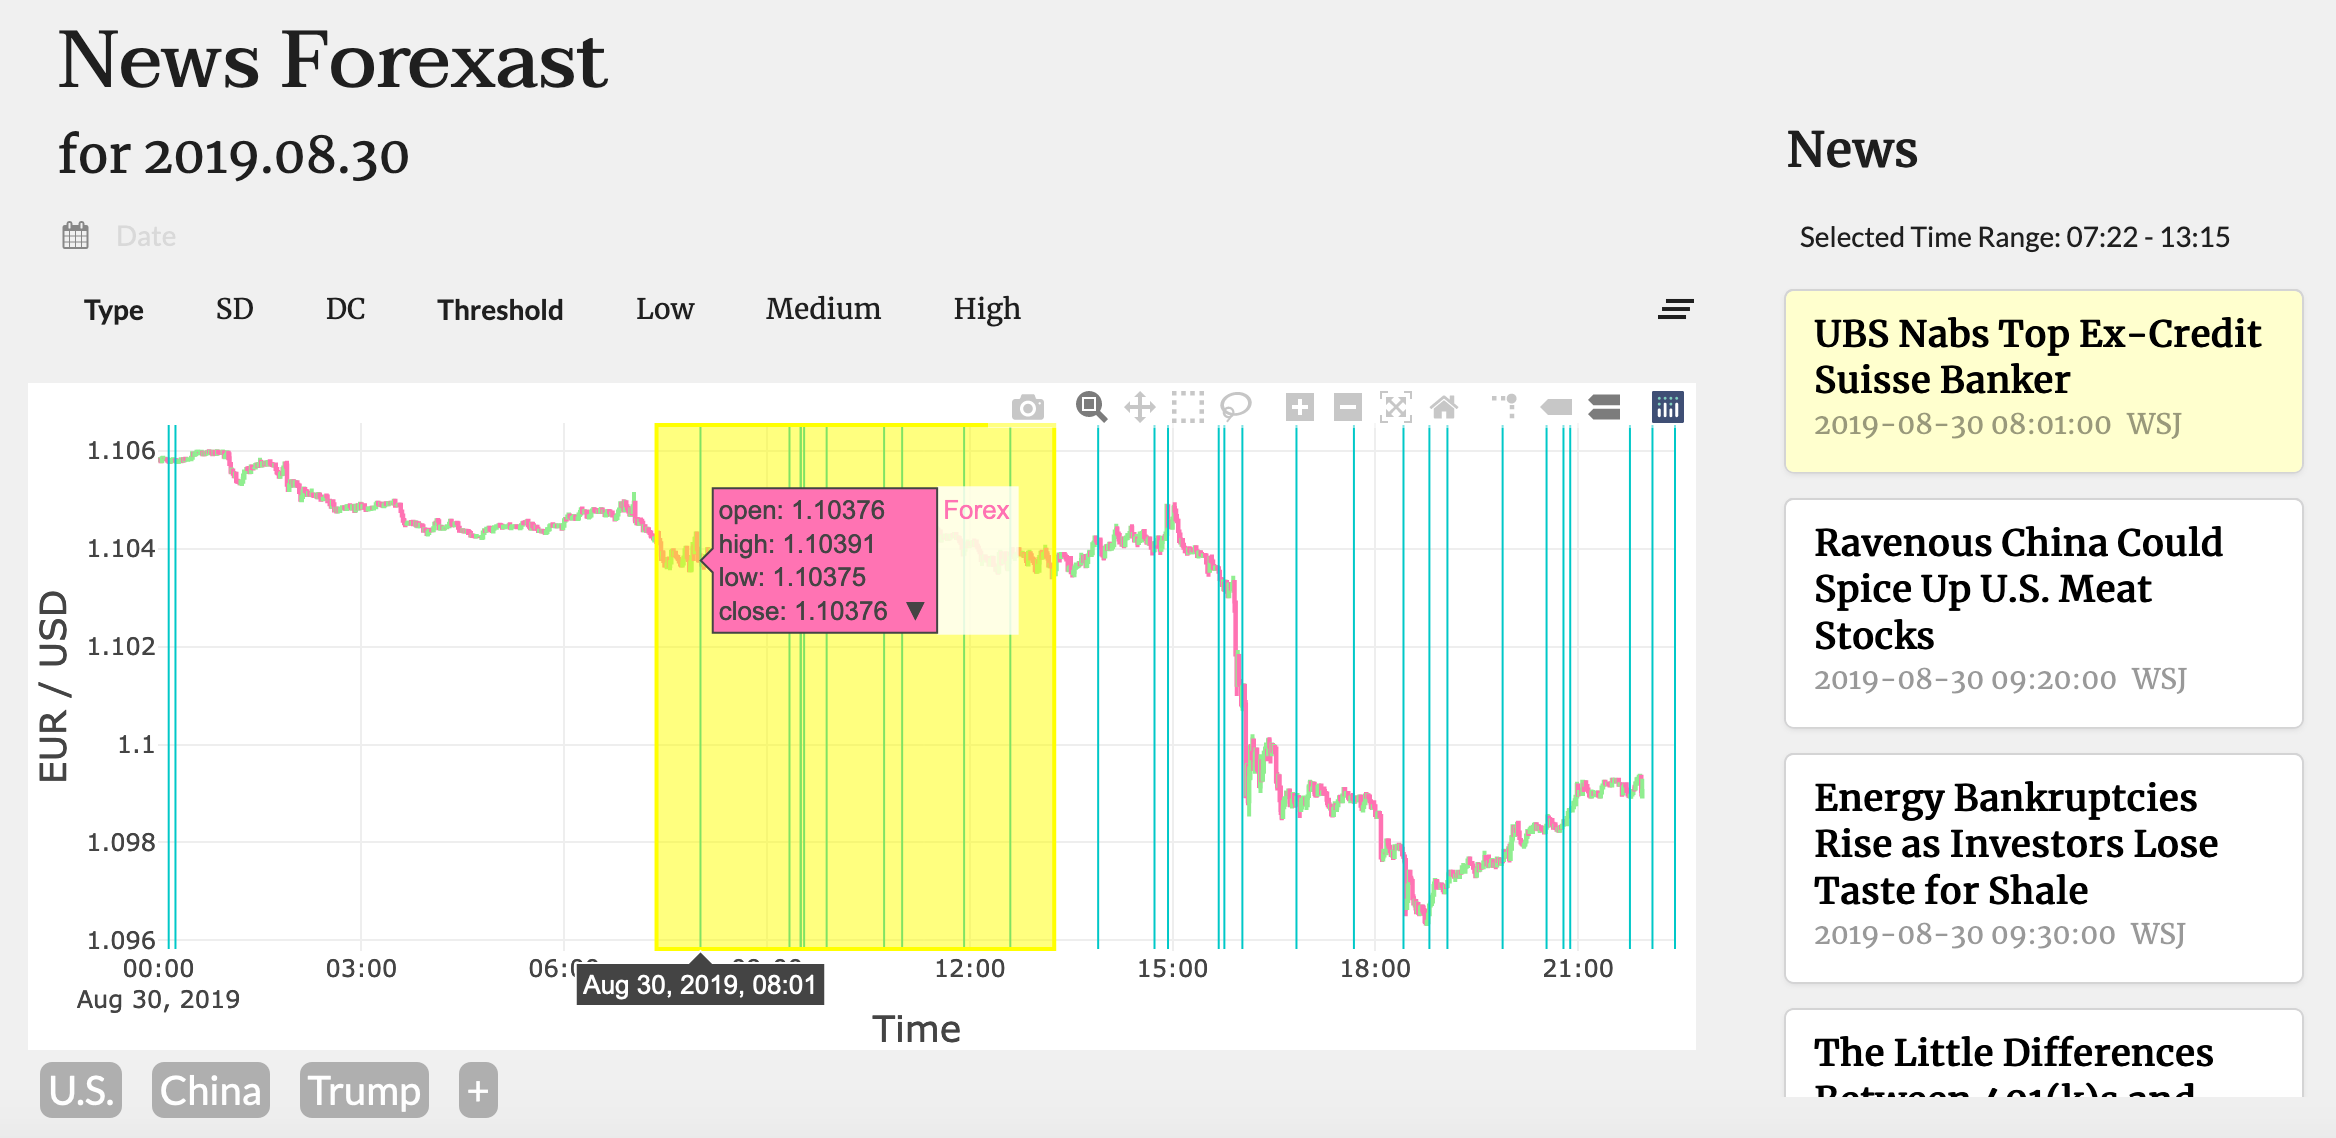
\includegraphics[width=\linewidth]{hover.png}
  \caption{Example of news being highlighted when the cursor hovers over the corresponding timeline on the chart. The yellow interval is the news selection range which can be decided by users.}
  \label{fig:hover}
\end{figure}

\subsubsection{Interactive Forex Chart}
The Forex prices are displayed by a standard candlestick chart, powered by Plotly graphing libraries.\footnote{\url{https://https://plotly.com/graphing-libraries/}}
Users can specify the date they are interested in with the calendar icon above the chart and then explore the chart freely by zooming in or dragging out the time frame they are interested.
Except for the Forex chart, the blue vertical lines correspond the news releasing time points. 
As shown in Figure~\ref{fig:hover}, the corresponding news in the right panel are highlighted if users hover over the corresponding blue line on the chart.
Users can also link to the original posts and websites by clicking on the news cards.
Moreover, users could easily spot specific time ranges they are interested in by double-clicking the start and end points of a period on the Forex chart (resulting in the yellow span in the figure); the news section in the right panel will change correspondingly according to the selected time span.


\subsubsection{Forex Event Identifier}
Users can specify event types (i.e., SD or DC) and the corresponding thresholds (i.e., Low, Medium, or High) with the bottoms below the date selection calendar, after which the algorithm output would be shown on the Forex chart as the gray dots for the SD events and the span lines for the DC events (e.g., see Figures~\ref{fig:SD} and~\ref{fig:DC} for examples of SD and DC events, respectively).
For example, users can specify August 30, 2019 and select the ``SD'' event with the ``Low'' threshold; from the upper panel of Figure~\ref{fig:SD}, users can tell that there exists a dramatic change during 14:30-16:30 on that day and can proceed to select a specific time range on the plot. 
In return, the news section would display related news such as ``Would Warren Buffett Buy Greenland?'' and ``Risky Seller Financing Flourishes Where Homes Are Cheapest.'' 
Note that once done with a specific setting, users can clear the setting with the ``clear all'' button on the top-right of the left panel in the system; also, a higher threshold (the lower panels in Figures~\ref{fig:SD} and~\ref{fig:DC}) locates less events.

\begin{figure}[h]
  \centering
  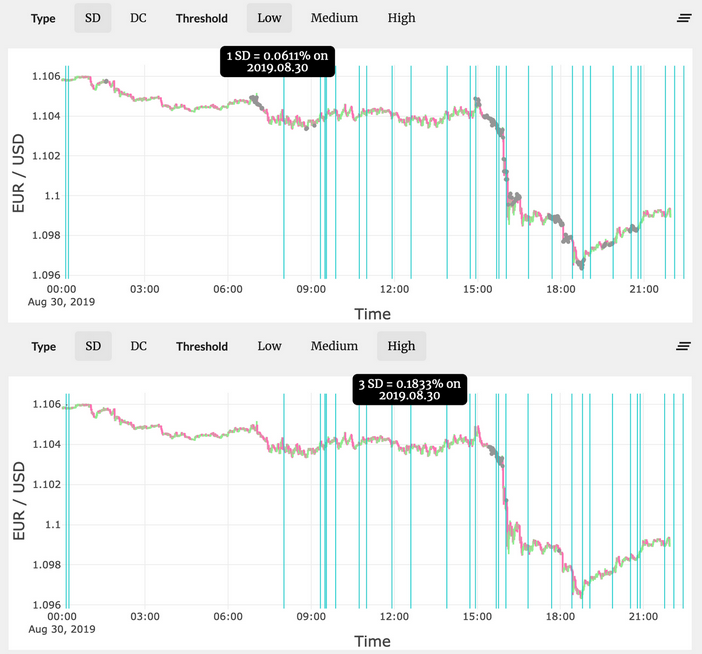
\includegraphics[width=\linewidth]{sd.png}
  \caption{Examples of displaying SD events on August 30, 2019. The upper panel is set to the ``Low'' threshold and the lower one is set to the ``High'' threshold.}
  \Description{}
  \label{fig:SD}
\end{figure}

\begin{figure}[h]
  \centering
  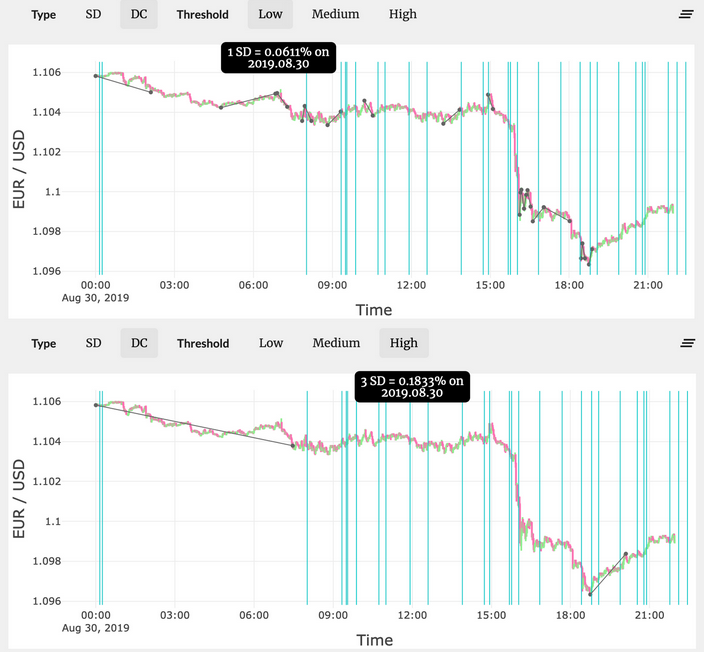
\includegraphics[width=\linewidth]{dc.png}
  \caption{Examples of displaying DC events on August 30, 2019. The upper panel is set to ``Low'' threshold and the lower one is set to ``High'' threshold.}
  \Description{}
  \label{fig:DC}
\end{figure}

\subsubsection{Customizable Keyword Filter
}
If users are interested in more specific news, they can use the tags under the plot to filter out news with selected keywords.
While we have placed several major keywords such as ``U.S.'' and ``Trump,'' as examples, users can customize their own tags by clicking the ``+'' button.
Figure~\ref{fig:keywords} shows the displayed news based one different keyword and time filters. 

\begin{figure}[h]
  \centering
  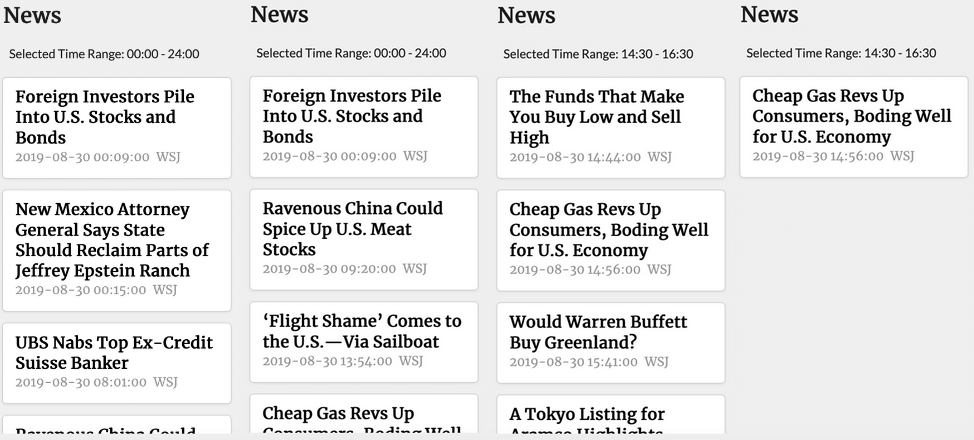
\includegraphics[width=\linewidth]{news.png}
  \caption{Examples of filtering news on August 30, 2019. From left to right are none, keyword: ``U.S.,'' time: '14:30-16:30', and both.}
  \Description{}
  \label{fig:keywords}
\end{figure}

\section{Case Study}\label{sec:case}

\begin{figure}[h]
  \centering
  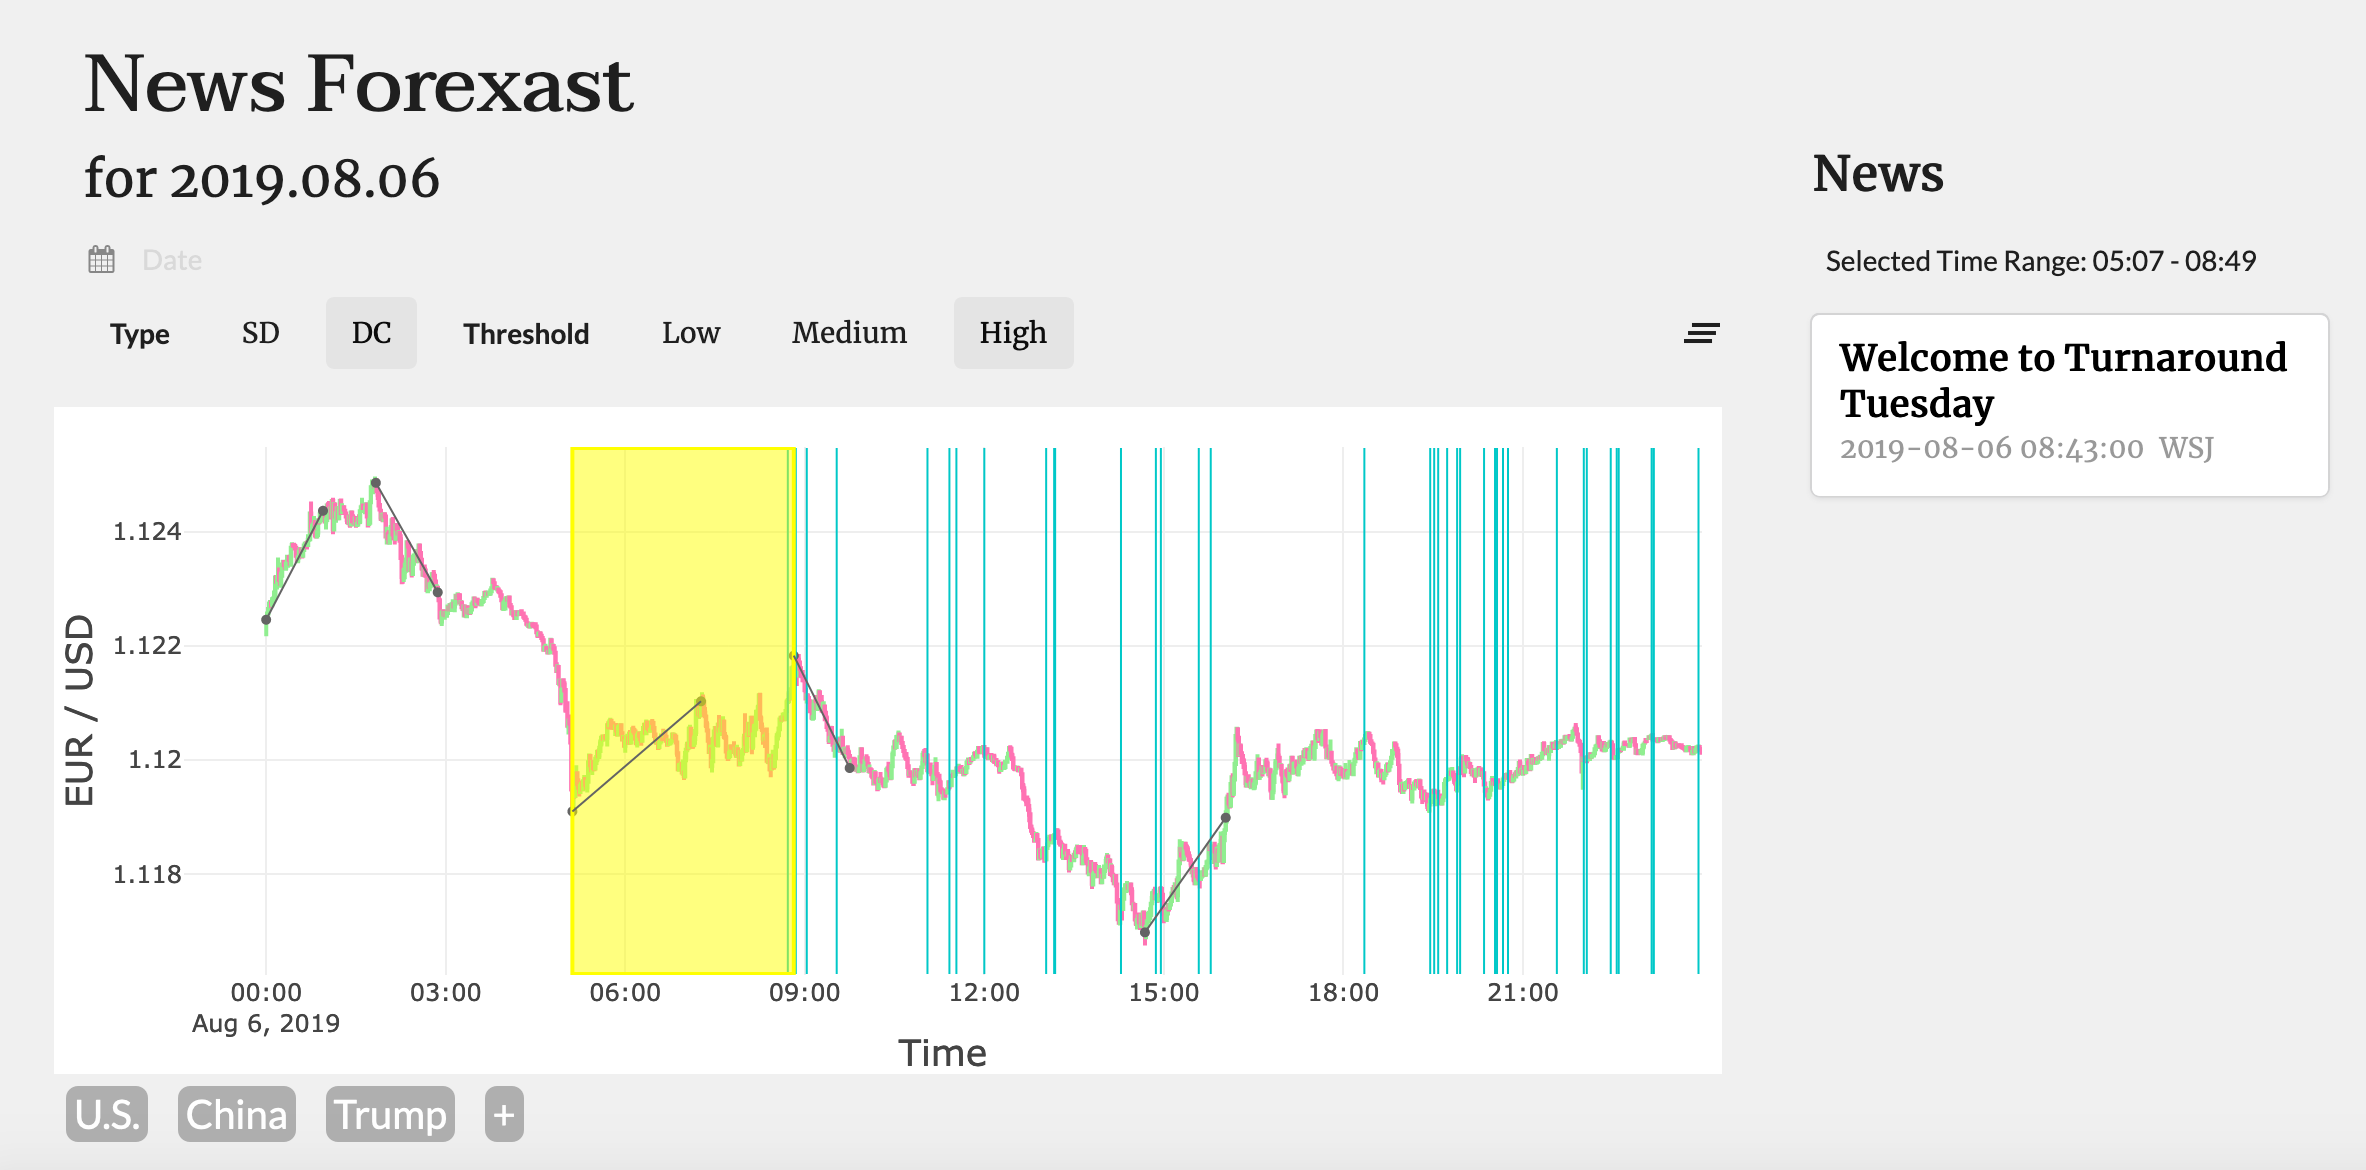
\includegraphics[width=\linewidth]{case.png}
  \caption{An example of case study.}
  \Description{}
  \label{fig:case}
\end{figure}

In this section, we provide an example that showcases the strong relation among events, news and Forex in Figure~\ref{fig:case}.
On August 6, 2019, we can see the news ``Welcome to Turnaround Tuesday'' released at 08:43, the time when an uptrend is about to end; note that the DC event with the High threshold shows that this uptrend starts at 05:07.
The news mentioned ``U.S. stock futures were in a decidedly better mood as Tuesday began than on Monday,'' indicating that U.S. stock is likely to rebound later, and thus causes appreciation on USD.
Then, the EUR/USD starts a downtrend from 08:49 to 14:41.
Note that if EUR/USD has a lower rate, it could be explained that USD has a relatively high value.

\section{Conclusion and Future work}\label{sec:conclude}
In this paper, we propose an interactive system, INForex, that aligns the presentation of the Forex data and the textual news data in a unified and time-aware manner.
By having the chart and related news side by side together, users, financial professionals, and amateur investors, can all understand the trend of Forex quicker and easier.
Beyond the presentation in this paper, We are now working toward to provide real-time news update in the system.
In addition, with the collected browsing behavior from users, we aim at providing more customized news feed via a personalized news recommender system by leveraging machine learning and natural language processing techniques.   

\section{Acknowledgments}



\bibliographystyle{ACM-Reference-Format}
\bibliography{reference}




\end{document}
\endinput
%%
%% End of file `sample-sigconf.tex'.
